\section{X-Window/GUI}
\textbf{programm-gesteuert}, \textbf{ereignis-gesteuert}(event-driven)\\
\textbf{X Window System:} Grundfunktionen der Fensterdarstellung\\
\textbf{Desktop Manager:} Hilfsmittel wie File-Manager, Papierkorb etc.\\
%X ist unabhängig von Window Manager/Desktop Manager\\
%Xlib: C Interface für X Protokoll\\
%X Toolkit: Software Schicht oberhalb Xlib, Standardbedienelemente

%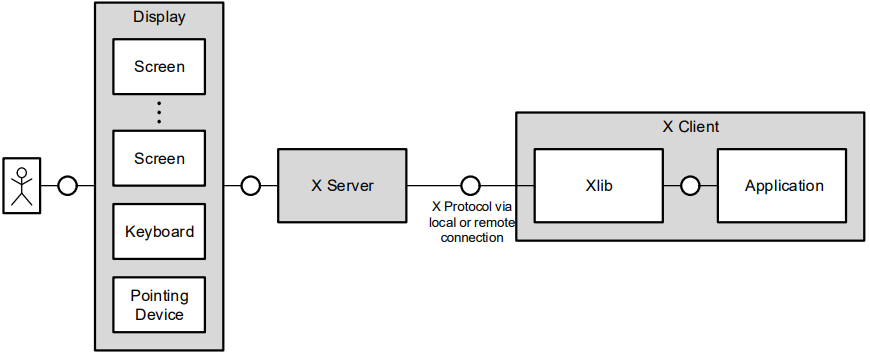
\includegraphics[scale = 0.3]{grafiken/x_uebersicht.PNG}\\
%Client: Will Display nutzen, lokal/remote\\

%\subsection{Window Manager}
%Verwaltung der sichtbaren Fenster, Umrandung, Knöpfe\\
%Clients geben WM Hinweise, wie sie angezeigt werden wollen $\rightarrow$ WM akzeptiert/modizifiert/ignoriert\\
%gilt als Client-Applikation mit Sonderrechten zur Fensterverwaltung\\
%auch Remote möglich

\subsection{Fensterverwaltung/Window Manager}
%2 Fensterklassen: \prgc{InputOutput}, \prgc{InputOnly}\\
Top-Level Window: Kind des Root-Window, gehören zu Applikation\\
%WM-Dekoration: hinter jedes Top-Level Window Extra-Fenster mit Knöpfen, Icons etc.\\
\textbf{Close-Button:} %WM sendet \prgc{ClientMessageEvent} an Applikation, Event hat in \prgc{data} Teil das Atom \prgc{WM_DELETE_MESSAGE} Registrierung des Clients:
\begin{minted}{C}
Atom atom = XInternAtom(display, "WM_DELETE_WINDOW", False);
XSetWMProtocols(display, window, &atom, 1);
\end{minted}

\subsubsection{Atom}
ID eines Strings, der für Meta-Zwecke benötigt\\
\prgc{Atom XInternAtom (Display*, char*, Bool only_if_exists)}\\
Übersetzt String in Atom auf angegebenen Display

\subsubsection{Properties}
WM liest/setzt Properties auf Fenster\\
Property über Atom identifiziert\\
Zu jedem Property gehören Daten wie Liste von Atomen, ein/mehrere Strings

\subsubsection{Protokolle Client$\leftrightarrow$WM}
Client-Registrierung: im Property \prgc{WM_PROTOCOLS} Liste der Atome der Protokollnamen speichern\\
\prgc{XSetWMProtocols(Display*, Window, Atom* first_arrayelem, int array_l)}

\subsection{X-Protocol}
Festlegung Formate für Nachrichten XClient$\leftrightarrow$Server\\
Events: z.B. Mausklicks, Maus traversiert Fenstergrenze\\
Für Requests: Nachrichtenbuffer auf Clientseite\\
Pufferleerung: wenn client auf Server wartet, Client-Request Reply benötigt, \prgc{XFlush()}
Für Events: doppelte Bufferung bei Server (checkt Netzwerk)/Client(nur selektierte Typen)

%\subsection{X-Ressource}
%z.B. Pixmap, Graphics-Context(GC)\\
%von Server gehalten, zugriff via ID\\
%default keine Bufferung für Hintergrundfenster, Neuzeichnung nötig (optional Server hat Hintergrundspeicher)\\
%\textbf{Pixmap:} Server-seitiger Grafikspeicher, von Client privat anlegbar\\
%\textbf{Graphics Context:} Liniendicke, Farbe etc., vor Aufruf einer Zeichenfunktion GC nötig, Mehrere GCs pro Client möglich\\

%\subsection{API}
%\begin{minted}{C}
%Display* XOpenDisplay(char* display_name)
%//display == null->Wert Umgebungsvar. DISPLAY genommen
%void XCloseDisplay(Display* display)
%XCreateWindow//Window ID als unsigned long zurück
%sfXDestroyWindow, XCreateSimpleWindow

%XMapWindow(Display*, window)//bestimmt, ob Fenster angezeigt
%//Fenster wird erst angezeigt, wenn Elternfenster angezeigt
%XMapRaised(Display*, window)//vor alle anderen Fenster
%XMapSubwindows(Display*, window)//zeigt alle Unterfenster
%//jedes angezeigtes Fenster -> Expose Event

%XUnmapWindow(Display*, Window)//alle Unterfenster auch
%XUnmapSubwindows(Display*, window)//nur Unterfenster
%//jedes versteckte Fenster -> UnmapNotify Event

%XSelectInput(Display*, Window w, long event_mask)
%//legt fest, welche Events ausgewählt werden

%While(1){
%XNextEvent(display, &event);
%switch (event.type){
%case Expose: ...
%case KeyPress: ...}}

%XCreateGC, XCopyGC, XFreeGC
%XDefaultGC//gibt default für Screen zurück
%\end{minted}

%\subsection{Farben}
%jeder Pixel: 3 Subpixel (rot/grün/blau)\\
%pro Farbanteil normalerweise 8 Bit verwendet $\rightarrow$ 24 Bit pro Farbe $\rightarrow$ $2^24=16$M Farben

%\subsubsection{colormap}
%z.B. 4 Bit Index für 24 Bit-Farbe, Reduktion gleichzeitig-darstellbarer Farben\\
%\begin{minted}{c}
%Colormap DefaultColormap(Display *, Screen)
%XCreateColormap, XFreeColormap
%XParseColor(Display*, Colormap, char* spezifi, XColor* out_p)//1
%//String zu Farbe in out_p machen
%XAllocColor(Display*, Colormap, Xcolor* color)//2
%//Farbe in Colormap anlegen
%XSetWindowAttributes//struct, mit Farben, Mauscursor etc.
%XChangeWindowAttributes(Display*, Window, unsigned long mask,
%XSetWindowAttributes*) //ändert in mask angegebene Attr.
%\end{minted}